
%\PARstart{U}{se} the force Luke...

\section{Introduction}\label{sec:GA:intro}

Innovative methodologies, such as multi-unit recording 
\citep{BrownKassEtAl:2004} and optical recording using voltage-sensitive dyes
\citep{GrinvaldHildesheim:2004,YangDoiEtAl:2000}, are enabling neuroscientists
to monitor the simultaneous activity of networks of neurons with a higher degree
of spatial and temporal accuracy than has been achieved previously at the
network level. At the same time, modeling biophysically-based neural networks
(BNN) is becoming more accessible and faster to run with modern computing
power. (By biophysically-based we mean models that include a description of
currents flowing through membrane ion channels, such as the Hodgkin-Huxley
model.)  To develop larger BNN's, with complex network behavior a number of
interrelated issues need to be considered: (a) what level of neuronal detail is
required to achieve observed phenomena in the network, (b) how do extrinsic and
intrinsic noise sources affect the model, and (c) how do we reliably constrain
the many free parameters in a model given limited experimental data.

\smallskip{} 

One set of approaches to constraining BNNs, denoted as ``bottom-up'',
is to construct them using detailed knowledge of specific neurons and
their membrane current properties. These bottom-up approaches to
neural modeling have been quite successful at representing single cell
models. They are, however, insufficiently sophisticated when it comes
to constraining the free parameters in small networks of neurons
\citep{GrillnerMarkramEtAl:2005,KochSegev:1998}, generally relying on
hand-tuning parameters. In contrast, the ``top-down'' approach to
constraining neural network models uses the output of the network
activity to infer the underlying model parameters. Such networks were
originally developed to be abstract feature detectors
\citep{Malsberg:1973} or simple nerve field projections
\citep{Amari:1980} based on general principles of neural processing.
Optimization and training algorithms for top-down network constraint
are highly efficient and generally involve a gradient-decent search
with a training method called back-propagation, where the output error
is calculated back through the network
\citep{RumelhartHintonEtAl:1986}. These algorithms are not applicable
to BNNs because the input/output relationships of Hodgkin-Huxley-type
models are not analytical, making them unsuitable for error
back-propagation.

\smallskip{} 

The particular challenges of constraining network parameters in BNNs
or ensembles of spiking neural networks, which have been discussed
previously \citep{EggertHemmen:2001,Brette:2007} focus on the
analytical methods characterizing the spike output
\citep{Victor:2005,KostalLanskyEtAl:2007,BrownKassEtAl:2004}. Inferring
the connectivity within a network requires a cost analysis of the
spiking output.  This has progressed from ensemble feature-based
methods
\citep{SameshimaBaccala:1999,DahlhausEichlerEtAl:1997,TheunissenSenEtAl:2000},
information theoretical approaches using maximum likelihood
\citep{YamadaMatsumotoEtAl:1996,Chichilnisky:2001,OkatanWilsonEtAl:2005,PaninskiPillowEtAl:2004},
evolutionary algorithm methods~\citep{TakahamaSakai:2005,Yao:1999},
and other non-linear approaches~\citep{Eblen-ZajjurSalasEtAl:1999}.
However, most of these efforts have been restricted to single neuron
models or networks of integrate-and-fire neural models rather than
BNNs.

\smallskip{} 

Genetic Algorithms (GAs) belong to a class of optimization algorithms
that mimic the process of evolution through natural selection. The
primary strength of GAs relative to other optimization techniques,
such as gradient-descent, is that GAs can avoid getting caught in
local minima \citep{Goldberg:1989,Whitley:1995}. Since
\citet{Holland:1975} first used GAs to evolve the connectivity and
synaptic weights of artificial neural networks, some other hybrid
methods have been proposed \citep{Yao:1999,Whitley:1995}. Existing
examples of biophysically-based neural models that have been
constrained using GAs are limited to single and multi-compartmental
single cell models
\citep{KerenPeledEtAl:2005,VanierBower:1999,VanDeEtAl:2008} or small
microcircuits \citep{TaylorEnoka:2004}.  They are generally regarded
as an effective method in automated
parameter-searches. \citet{KerenPeledEtAl:2005} used intracellular
recordings from a cortical pyramidal cell to constrain the membrane
conductances of a multi-compartmental model.  The synaptic input noise
was filtered out, enabling the model data to be fit to experimental
recordings. \citet{TaylorEnoka:2004} used a microcircuit of spinal
motor units that was trained using feature-based analysis of the
output to fit the membrane and synaptic parameters.  Ongoing work in
BNN modeling \citep{VanierBower:1999,VanDeEtAl:2008} is making headway
in removing the hand-tuning of parameters, but the application to
medium and large-scale networks may require more techniques from the
top-down methods in cost analysis and optimization algorithms.

\smallskip{} 

This section of the thesis investigates the application of GAs in
constraining synaptic parameters in a topographically-ordered BNN, using the
example of a network in the auditory brainstem. The design of the GA, outlined
in the Methods, includes the specification of a cost function that measures how
well the model network reproduces the target data. We assess three alternate
cost functions derived, in different ways, from the output of neural responses
in the network. Each cost function is based on measures of (1) spike timing, (2)
instantaneous firing rate, or (3) average intracellular voltage. Surrogate data
from a randomly generated network model served as our target and the ability of
the algorithms to find the known neural parameters was assessed. To analyze the
robustness of the cost functions to synaptic noise and the effects of
trial-to-trial variability we incorporated these effects into the model.

\subsection{Stellate Microcircuit of the Cochlear Nucleus}\label{sec:GA:stell-micr-cochl}

The network used as the basis for optimising BNNs lies in the cochlear
nucleus (CN, Figure~\ref{fig:GA:CNdiagram}), which is the gateway
between the peripheral auditory system and the central nervous system,
with six distinct pathways to higher auditory nuclei
\citep{CantBenson:2003}. The principle neurons in the circuit are the
T-stellate (TS) cells, in the ventral cochlear nucleus (ventral CN,
Figure~\ref{fig:GA:CNdiagram}), which project to the inferior
colliculus.  They provide a robust spectral representation of sound
and are implicated in forming part of the main `what' pathway for
auditory information \citep{YoungOertel:2004}. Experimental evidence
indicates that synaptic inputs from inhibitory interneurons play a
critical role in modulating the input-output response properties of TS
neurons
\citep{FerragamoGoldingEtAl:1998,NeedhamPaolini:2006,PaoliniClareyEtAl:2005}.
The neurons TS, together with their inhibitory interneurons and
afferent inputs, form a microcircuit, which we have taken as our
example network.


 \begin{figure}[pt!]
\centering
   \resizebox{5in}{!}{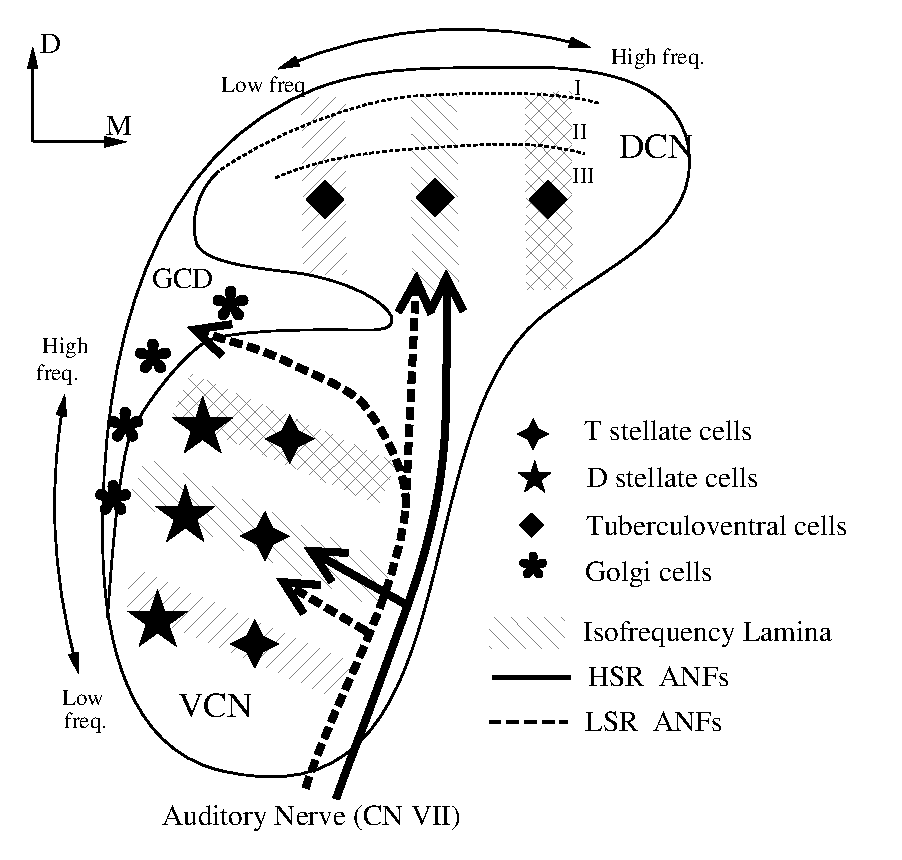
\includegraphics{CNConnections3}}
   \caption{Diagram of the mammalian cochlear nucleus. Auditory nerve
    fibers (ANFs) sensitive to particular frequencies project to the
    cochlear nucleus (CN) in a tono-topically organized fashion and
    bifurcate to innervate both the ventral CN and dorsal CN\@. The
    CN comprises two main divisions, ventral and dorsal CN, plus an
    outer layer of small cells known as the granule cell domain
    (GCD). Type I ANFs are characterized into two groups based on
    their spontaneous rate: high (HSR, solid line) and low (LSR,
    dashed line). Only LSR and smaller type II ANFs project to the
    GCD\@.  Golgi cells in the GCD are the only known source of
    GABAergic cells within the ventral CN, and it is presumed that
    they synapse with TS and DS cells
    \cite{FerragamoGoldingEtAl:1998}. Glycinergic D-stellate cells
    (DS) project to wide areas of the ventral CN, dorsal CN, and
    contralateral CN\@. DS cells are broadly tuned and respond best
    at the onset of a tone, with a small number of precisely timed
    spikes, and respond strongly to broad-band noise.  In the deep
    layer of the dorsal CN, tuberculo-ventral (TV) cells provide a
    narrow-band on-frequency source of glycinergic inhibition to the
    ventral CN\@. These neurons respond poorly to clicks and
    broad-band noise, due to wide-band inhibition from DS cells
    \cite{SpirouDavisEtAl:1999}.}
\label{fig:GA:CNdiagram}

 \end{figure}
 \clearpage


\begin{figure}[t!]
\centering
\figfont{A}\hfill\\
\resizebox{3in}{!}{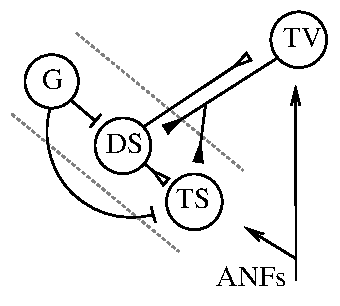
\includegraphics{SimpleCircuit3}}
\figfont{B}\hfill\\
\resizebox{3in}{!}{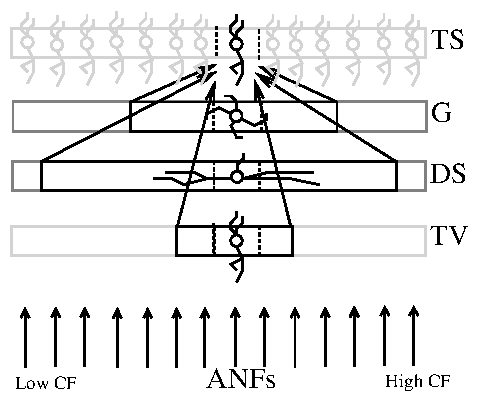
\includegraphics{NetworkProjections3}}
\caption{(A) Stellate microcircuit showing synaptic interaction within one
  iso-frequency lamina of the ventral CN (dotted lines) and TV cells of the
  dorsal CN\@. Excitatory synapses from ANFs (arrows) are modulated within the
  network by glycinergic (triangle) and GABAergic (T) inputs. (B)~ANFs are
  ordered into a wide range of frequency channels that are mapped to the ventral
  CN and dorsal CN in an orderly, tono-topic fashion. Topographic organization
  of lateral connections in the CN stellate network shows the range of inputs to
  TS cells from Golgi, DS and TV cells. Dendritic morphologies of cells
  characterize the range of ANF inputs and hence determine their frequency
  response. ANF input to TS and TV cells are restricted to one iso-frequency
  lamina, whereas DS dendrites span 1/3 of the ventral CN\@. DS cells' axonal
  plexus typically covers 1/3 of the ventral CN and one half of the dorsal CN,
  giving them a strong influence throughout the CN
  \cite{ArnottWallaceEtAl:2004}.}
\label{fig:GA:MicroCN}
\end{figure}

\smallskip{} 

The tonotopic organization of the auditory pathway (i.e.\ the
continuous mapping of sound frequency to place of resonance in the
cochlea) is transferred to the CN through the population of auditory
nerve fibers (ANFs)
\citep{Lorente:1981}. Figure~\ref{fig:GA:CNdiagram} shows that ANFs
enter the brainstem ventrally and bifurcate, so that each fiber sends
axonal collaterals to the ventral and dorsal sections of the cochlear
nucleus, to organized iso-frequency lamina. ANFs are categorized into
high spon\-taneous rate (HSR, Figure~\ref{fig:GA:CNdiagram} solid line)
and low spontaneous rate (LSR, Figure~\ref{fig:GA:CNdiagram} dashed
line) fibers. LSR fibers have a higher threshold than HSR fibers and
do not saturate in response to loud sounds.

\smallskip{} 

The connectivity of the cell types involved in the stellate
microcircuit is shown in Figure~\ref{fig:GA:MicroCN}. Fast,
glycinergic inhibition from tuberculoventral (TV) cells and D-stellate
cells (DS, Figure~\ref{fig:GA:CNdiagram}) is involved in modulating
the firing rate and spike interval variability in TS cells
\citep{FerragamoGoldingEtAl:1998,WickesbergOertel:1993}. TV cells in
the deep layer of the dorsal CN, provide a delayed narrowband
inhibition to TS and DS cells in the ventral CN\@.  The dendrites of
DS cells cover 1/3~of the cross-frequency axis in the CN, contributing
to this cell's wide frequency response. In turn this cell is
responsible for altering the frequency responses in TS and TV cells
\citep{SpirouDavisEtAl:1999}. DS cells are coincidence detectors and
have a precisely timed onset response that affects the temporal
properties of TS cells
\citep{PaoliniClareyEtAl:2005,RhodeGreenberg:1994a} and completely
inhibit TV cell responses to loud clicks
\citep{SpirouDavisEtAl:1999}. GABAergic inhibition from Golgi cells
(Figure~\ref{fig:GA:CNdiagram}) modulates the level of excitation
necessary to reach threshold for all CN cells
\citep{CasparyBackoffEtAl:1994,FerragamoGoldingEtAl:1998}. Feedback
circuits from the olivary complex to the ventral CN are also known to
use GABA as a neurotransmitter \citep{SaintMorestEtAl:1989}, however
this is not included in the model.

\smallskip{} 

\section{Methods}

\subsection{Genetic Algorithm Implementation }

For a model constraining problem, genetic algorithms work by searching
across successive generations of models for the model that is
``fittest'' in the sense that it best reproduces some user supplied
data. Each generation of models is obtained from the previous one by
using fitness-based selection criteria to create new models from
existing members of the population. In this process a model is
represented by a genome, which is the result of mapping the model
parameters into binary strings and concatenating them together. Each
population of genomes is evaluated for fitness using a carefully
tailored cost-function, better fitness increases the probability that
a genome will contribute to the next population.  The basic principles
of genetic reproduction, viz.\ crossover operation and mutation, are
used to generate new genomes from selected existing genomes. A
crossover operation breaks two genomes at a random location and swaps
their tail portions to create two new genomes. A mutation is a random
bit reversal in a genome. Crossover operations ensure that there is
adequate mixing of the best performing genomes in the population and
mutations are introduced to ensure diversity. The best members of the
population are usually copied (cloned) in the new population.

\smallskip{} 

In this work, all GA simulations ran with 100~genomes in each
population and evolved for 200~generations. From each population, a
new population was created by cloning the five best genomes and
performing the following procedure for the remaining 95~genomes.
Candidate genomes for crossover were randomly selected based on their
fitness, using the roulette-wheel selection probability function,
where each score was linearly scaled so that the probability of
selection, $P_i$, is:
\begin{equation} \label{eq:GA:1} 
P_{i} =1 - \frac{g_{i} }{G}
\end{equation}
\noindent where $g_i$ is the genome's cost-function score, and $G$ is
the sum of all genome scores in the current population (note that the
sign in front of $g_i$ is negative here, instead of the conventional
positive, because we use cost-functions corresponding to an error
term, so that smaller values of $g_i$ imply greater
fitness). Following selection of a genome, crossover occurred with a
strictly different selected genome, with probability 0.95.
Alternatively the selected genome was cloned, with probability 0.05.
For the group of 95~genomes, a random bit mutation was implemented
with probability 0.01. The best performing genome string at the end of
the 200th generation was declared the winner.

\smallskip{} 

Parameters that were optimized were the synaptic weights, number of
synaptic connections per neuron and a parameter describing the spatial
variance of connections (details are given in the
section~\ref{sec:GA:connectivity} Connectivity). The genome encoding
scheme, shown in Table~\ref{tab:GA:Genome}, describes the number of bits
used for each parameter and the range of values that each parameter
could take.  For example, the first parameter in Table~\ref{tab:GA:Genome},
$w_{{\rm ANF}\to{\rm TS}}$ models the strength of synapses from ANF to
TS cells. It was encoded over the range 0.0-0.0051 $\mu$S using 8~bits
by assigning 0b00000000~to 0.0~and 0b11111111~to 0.0051, and linearly
interpolating all values within the range. This procedure was used for
all parameters where the unit step was either 0.0001 $\mu$S for weight
parameters or 1 (synaptic connection or frequency channel) for all
others. The number of bits representing each parameter was chosen so
that the maximum value lay outside of known physiological
values. Genomes were formed by concatenating all these parameter bit
strings in the order given in Table~\ref{tab:GA:Genome}.

\smallskip{}

To test the application of GA's for optimizing parameters of a BNN, a
network with a known set of parameters was created, this is referred
to as the target network.  This allowed us to assess the GA by how
well the algorithm was able to recover the target parameters. The
target parameters were randomly selected from within the physiological
range of values and given in Table~\ref{tab:GA:Genome}.  Target data were
generated from the target network and used as training data for the GA
by incorporating them in an error-based cost function.  A notch-noise
stimulus (described under Stimulus Generation) was chosen to present
to the network as it produced a spectrally rich response that was
spread over the whole frequency range of the target network.  Figure
3A shows a spike raster plot for all TS cells to a presentation of the
notch noise stimulus. The vertical axis is arranged according to the
frequency to which the neuron is most sensitive (the center
frequency). There is a clear reduction in the firing rate
corresponding to the stop band in the
notch-noise. Figure~\ref{fig:GA:Costfunctions}B illustrates response
to 250~repetitions for a single TS cell in the center of the network,
at the rising edge of the notch (arrow in
Figure~\ref{fig:GA:Costfunctions}A).

\begin{table}[tp]
 \centering
 \caption{Network Parameter-to-Genome Encoding Scheme}\label{tab:GA:Genome}
 \begin{tabularx}{\textwidth}{lcccXX}
\hline
  &           Parameter           & Binary Bits & \multicolumn{2}{c}{Range} & Target Value \\[0.5ex]\hline
1  & $w_{{\rm ANF}\to {\rm TS}} $  &      8      & 0.0 &       0.0051        & 0.00270 \\ %\hline
2  & $n_{{\rm LSR}\to {\rm TS}} $  &      5      &  0  &         31          & 7 \\ %\hline
3  & $n_{{\rm HSR}\to {\rm TS}} $  &      5      &  0  &         31          & 22 \\ %\hline
4  & $w_{{\rm ANF}\to {\rm DS}} $  &      8      & 0.0 &       0.0051        & 0.00178 \\ %\hline
5  & $n_{{\rm ANF}\to {\rm DS}} $  &      6      &  0  &         63          & 27 \\ %\hline
6  & $n_{{\rm HSR}\to {\rm DS}} $  &      6      &  0  &         63          & 59 \\ %\hline
7  & $w_{{\rm ANF}\to {\rm TV}} $  &      8      & 0.0 &       0.0051        & 0.00091 \\ %\hline
8  & $n_{{\rm LSR}\to {\rm TV}} $  &      5      &  0  &         31          & 13 \\ %\hline
9  & $n_{{\rm HSR}\to {\rm TV}} $  &      5      &  0  &         31          & 16 \\ %\hline
10 & $w_{{\rm LSR}\to {\rm GLG}} $ &      8      & 0.0 &       0.0051        & 0.00150 \\   %\hline
11 & $n_{{\rm LSR}\to {\rm GLG}} $ &      5      &  0  &         31          & 16 \\   %\hline
12 &  $w_{{\rm DS}\to {\rm TS}} $  &      8      & 0.0 &       0.0051        & 0.00028 \\ %\hline
13 &  $n_{{\rm DS}\to {\rm TS}} $  &      5      &  0  &         31          & 14 \\ %\hline
14 &  $s_{{\rm DS}\to {\rm TS}} $  &      6      &  0  &         63          & 15 \\   %\hline
15 &  $w_{{\rm TV}\to {\rm TS}} $  &      8      & 0.0 &       0.0051        & 0.00040 \\ %\hline
16 &  $n_{{\rm TV}\to {\rm TS}} $  &      5      &  0  &         31          & 12 \\ %\hline
17 &  $s_{{\rm TV}\to {\rm TS}} $  &      5      &  0  &         31          & 3 \\   %\hline
18 & $w_{{\rm GLG}\to {\rm TS}} $  &      8      & 0.0 &       0.0051        & 0.00022 \\ %\hline
19 & $n_{{\rm GLG}\to {\rm TS}} $  &      5      &  0  &         31          & 7 \\ %\hline
20 & $s_{{\rm GLG}\to {\rm TS}} $  &      5      &  0  &         31          & 3 \\   %\hline
21 &  $w_{{\rm DS}\to {\rm TV}} $  &      8      & 0.0 &       0.0051        & 0.00042 \\ %\hline
22 &  $n_{{\rm DS}\to {\rm TV}} $  &      6      &  0  &         63          & 18 \\ %\hline
23 &  $s_{{\rm DS}\to {\rm TV}} $  &      6      &  0  &         63          & 8 \\   %\hline
24 &  $w_{{\rm TV}\to {\rm DS}} $  &      8      & 0.0 &       0.0051        & 0.00016 \\ %\hline
25 &  $n_{{\rm TV}\to {\rm DS}} $  &      6      &  0  &         63          & 7   \\ %\hline
26 &  $s_{{\rm TV}\to {\rm DS}} $  &      6      &  0  &         63          & 3 \\   %\hline
27 &  $o_{{\rm DS}\to {\rm TV}} $  &      5      &  0  &         31          & 3 \\ %\hline
28 & $w_{{\rm GLG}\to {\rm DS}} $  &      8      & 0.0 &       0.0051        & 0.00246 \\   %\hline
29 & $n_{{\rm GLG}\to {\rm DS}} $  &      5      &  0  &         31          & 7 \\ %\hline
30 & $s_{{\rm GLG}\to {\rm TDS}} $ &      5      &  0  &         31          & 5 \\[0.5ex]\hline
\end{tabularx}\\
 \footnotesize{Units of weights are $\mu$S. $n$ and $s$ parameters are
   unitless integers. The resolution of weight parameters were set to
   0.0001 $\mu$S and other parameters to 1.}
\end{table}




\subsection{Cost functions}\label{sec:GA:cost-functions}

At the core of a GA optimization is a cost function, which is given,
here, by an error measure of some observable output of a trial network
against the output of the target network. In this work, the total cost
function score is calculated using the output of all cells in the
network.  Three different cost functions were investigated that were
based on experimental observables: spike times, instantaneous firing
rates, and intracellular voltages.


\begin{figure}[pt!]
  \begin{center}
%\setlength{\unitlength}{1pt}
    \resizebox{2.5in}{!}{%
\begin{picture}(206,108)(0,0)
  \put(0,0){\includegraphics[bb=98 523 304 631,clip]{Figure3}}
  \put(25,48){\thicklines\vector(1,0){10}}
  \end{picture}}%
    \resizebox{2.5in}{!}{\includegraphics[bb=98 411 304 523,clip]{Figure3}}\\
    \vspace{0.1in}\resizebox{5in}{!}{\includegraphics[bb=98 173 504 411,clip]{Figure3}}
\end{center}
  \caption{Cost function measures derived from the output of the CN
    stellate network. (A) Dot raster of TS cell spikes only during a
    presentation of the notch noise stimulus. A rough trace shows
    the relative location of the 30-dB notch in a broadband spectrum
    from 0.2~to 30 kHz. Frequency scale is determined by the
    Greenwood function for the cat \cite{Greenwood:1990}. (B) The
    reference spikes for a TS cell in the middle of the `target'
    network (CF 3.45kHz) from 250 repetitions of the stimulus are
    shown. This cell is placed at the edge of the spectral notch
    (arrow in A.). (C) PSTH response of the same TS cell used in B
    (bin width 0.25~ms, reps. 250). Note the regularly-spaced peaks
    at the start of the stimulus due to the TS cells' chopper
    response characteristics. Irregular peaks throughout the
    stimulus are due to temporal features of the notch noise
    captured by the auditory filter at this frequency. (D) PSTH of
    the same cell as in C using only 25 repetitions. The IFR cost
    function normalizes the reference PSTHs and calculates a mean
    squared error between reference and test PSTHs for every cell in
    the network. (E) Average intracellular voltage, smoothed from
    250 repetitions, for the same TS cell. There is some similarity
    with the PSTH in C, particularly the location of the peaks but
    contains subthreshold effects. (F) Average intracellular voltage
    using 25 repetitions is more variable than E since single action
    potentials can distort the trace.}
\label{fig:GA:Costfunctions}
\end{figure}
\clearpage

\subsubsection{Spike Timing Cost Function}\label{sec:GA:spike-timing-cost-fn}


Spike times give accurate temporal information but are limited by a
focus on individual stimulus presentations, which may contain various
sources of noise and trial-to-trial variability. The metric we used
for comparing trial and target spike trains applied a cost based on
relative timing of spikes, for a review see \citet{Victor:2005}.

\smallskip{}

The spike timing (ST) cost function was defined as:
\begin{equation} \label{eq:GA:2} 
\Psi _{{\rm ST}} = \frac{1}{N_{{\rm ST}}
  } \sum _{i=1}^{M}\sum _{j=1}^{R}\mathop{\min}\limits_{k}
  \left(D\left(x_{ij} ,x_{ik}^{*} \right)\right)
\end{equation}
\noindent where $N_{{\rm ST}} =R\times M$ is a normalization factor,
$M=240$~is the number of neurons in the network, $R=25$ is the total
number of stimulus repetitions, $x_{ij}$ is the vector containing the
spike times of the trial network for stimulus repetition $j$ produced
by neuron $i$, and $x_{ik}^{*}$ is the vector containing the spike
times of the target network for the stimulus repetition $k$ produced
by neuron $i$.  The units for $\Psi_{{\rm ST}}$ are ms per cell per
spike train for 60~ms duration spike trains but will be milliseconds
for the remainder of the study. $D(x_{ij} ,x_{ik}^{*})$ is the
difference measure between trial and target network spike trains as
found by dynamic programming.  Dynamic programming is a method for
analyzing sequential processes \citep{Denardo:1982} and was applied to
find the minimum distance between two spike trains, as illustrated in

\begin{figure}[t!]
 \resizebox{3in}{!}{gfx/DynamicSpikeMetric_v2.TpX}
  \caption{Spike timing cost function measure computed using a
    dynamic programming algorithm. A minimum distance matrix between
    the \textit{target} set of spike times and a \textit{trial} set
    of spike times (from the same cell in the network, $i$, is
    traversed to find the minimum cumulative path of timing
    errors. Arrows indicate the possible combinations of spike time
    errors. For every cell, each repetition in the trial set, $j$,
    is compared against 25 repetitions, $k$, in the training data to
    find the best fit and to minimize penalties for missing or
    additional spikes.}
\label{fig:GA:DynSpikeMetric}
\end{figure}

\smallskip{}

Figure~\ref{fig:GA:DynSpikeMetric}.  In this process, a trial spike train, $x_{ij}$,
was mapped onto a target spike train, $x_{ik}^{*}$, by a process of
realignment, without specifically considering insertion or deletion of
spikes. Insertion and deletion of spikes require additional penalties
and have been used in single spike trains
\citep{VictorGoldbergEtAl:2007,Aronov:2003}.  The cost associated with
a spike in the trial network and a spike in the target network was
measured as the time difference between the spikes. The spikes to
select for comparison were chosen such that the overall cost was
minimized.

\smallskip{}

We chose the minimum value of $D(x_{ij} ,x_{ik}^{*} )$ over 25~target
network spike-time vectors, $x_{ik}^{*}$, $k=1,\dots,25$, to reduce
the effect of output randomness, it was limited to 25~vectors to
obtain a reasonable computational load.  In the case where a trial
network produces no output spikes, $D(x_{ij} ,x_{ik}^{*})$ is the sum
of the target spike times, no target neurons produced empty spike
trains.

\smallskip{}

To illustrate the behavior of this cost function in the ideal case,
where ANF inputs to the trial network are the identical those used in
the 25~repetitions of the target data and the target network
parameters are used, the value of $\Psi_{{\rm ST}}$ is zero. The
maximum value of $\Psi_{{\rm ST}}$ observed in this study was
approximately 360~ms.  For an example trial network that produces the
correct number of spikes for each neuron but with an average spike
timing error of 1~ms, given that the average number of spikes per
train is 9, the cost function would be $\Psi_{{\rm ST}}=9$~ms per
spike train.



\subsubsection{Instantaneous Firing Rate (IFR) Cost Function}\label{sec:GA:inst-firing-rate-cost-fn}


The peri-stimulus time histogram (PSTH) has been an effective tool for
classifying the stimulus-induced time-varying firing rate in many
neurons including auditory neurons
\citep{BlackburnSachs:1989,SmithRhode:1989}.  When measured using very
short time bins ($<$1~ms), the estimated firing rate is called the
instantaneous firing rate (IFR).  The IFR cost function was obtained
from the mean squared error between each neuron's PSTH, $r_{i} $, and
the corresponding target neuron's PSTH, $r_{i}^{*} $, it was
normalized to obtain a firing rate (spikes per ms) error per stimulus.

\smallskip{}

The IFR cost function is defined as:
\begin{equation} \label{eq:GA:3} 
\Psi_{{\rm IFR}} =\frac{1}{T_{{\rm IFR}}
  } \sqrt{\frac{1}{M} \int_{i=1}^{M}\frac{1}{B} \int _{n=1}^{B}(r_{i}
    (n)-r_{i}^{*} (n))^{2} },
\end{equation}
\noindent where $B$ is the number of bins in the PSTH, $M$ is the
number of cells in the network, $T_{{\rm IFR}}=R\times W$ is a
normalization factor, $R$ is the number of trial repetitions
($R=25$~was used in this study), and $W$ is the bin width of the
PSTH\@. The units for $\Psi_{{\rm IFR}}$ are spikes per millisecond
per stimulus per neuron, but we shall use spikes per ms for the
remainder of this study.

\smallskip{}

To increase robustness of the IFR cost function to input and
trial-to-trial variability, target data from 250 repetitions was used
to generate a higher resolution set of target PSTHs $r_{i}^{*}$ and
scaled by 0.1~to match the trial PSTH repetition
number. Figure~\ref{fig:GA:Costfunctions}D shows an example of a TS cell's PSTH
produced from 250~repetitions of a notch noise stimulus. Similarly,
Figure~\ref{fig:GA:Costfunctions}E shows the same cell but with 25 repetitions. The
smoother PSTH of $r_{i}^{*}$ is evident in Figure~\ref{fig:GA:Costfunctions}D when
compared to the 25 repetitions in Figure~\ref{fig:GA:Costfunctions}E. Each PSTH is
60~ms in duration (50~ms stimulus then 10~ms silence) and discretized
using a bin width of $W=0.25$~ms (total number of bins $B=241$).

\smallskip{}

While the minimum value that $\Psi_{{\rm IFR}}$ can attain is zero, in
practice it will be greater than zero even when the trial network
exactly matches the target because the numbers of repetitions used to
create $r_{i}^{*}$ and $r_{i}^{}$ are different (250 and 25
respectively). The maximum $\Psi_{{\rm IFR}}$ value observed in this
study was approximately 0.5~spikes/ms per stimulus per neuron. For a
trial network, if the average PSTH error is 10~spikes over all bins,
then $\Psi_{{\rm IFR}} $ is approximately 0.2~spikes/ms.

\subsubsection{Average Intracellular Voltage (AIV) Cost Function}\label{sec:GA:aver-intr-volt-cost-fn}

Intracellular voltage responses reflect the influence of excitatory
and inhibitory inputs on a neuron. This may be a more reliable way of
determining the strength of synaptic inputs, since spike times and
PSTHs do not convey any information about the subthreshold activity of
a neuron. The intracellular voltage waveform has been used to
constrain single neural models with deterministic current inputs and
no synaptic noise \citep{KerenPeledEtAl:2005,VanierBower:1999}. In the
cochlear nucleus, averaging intracellular voltages over many
repetitions has been used to categorize physiological responses,
especially different stellate cells
\citep{PaoliniClareyEtAl:2004,PaoliniClareyEtAl:2005}.

\smallskip{}

The AIV cost function is defined using the mean-squared error between
averaged IV waveforms of each trial neuron, $\bar{v}_{i}^{}$, and the
corresponding target averaged IV waveform, $\bar{v}_{i}^{*}$, it is
normalized to obtain a voltage (mV) error per neuron per stimulus.

\smallskip{}

The AIV cost function is defined as:
\begin{equation} \label{eq:GA:4} 
\Psi_{{\rm AIV}} =\frac{1}{R}
  \sqrt{\frac{1}{M} \int_{i=1}^{M}\frac{1}{N}
    \int_{n=1}^{N}(\bar{v}_{i} (n)-\bar{v}_{i}^{*} (n))^{2} }
\end{equation}
\noindent where $N$ is the number of points in the IV waveform, $M$ is
the number of cells in the network, and $R$ is the number of
repetitions.

\smallskip{}

Figures~\ref{fig:GA:Costfunctions}F and~\ref{fig:GA:Costfunctions}G show examples of averaged IV
waveforms, $\bar{v}$, from a TS cell averaged over 25~or
250~repetitions, respectively, illustrating the reduction in
trial-to-trial variation with more repetitions. Action potentials were
clipped at 0~mV so that irregular peak heights did not affect the
average waveform.

\smallskip{}

The minimum value of $\Psi_{{\rm AIV}}$ is zero.  Similar to
$\Psi_{{\rm IFR}}$, in practice the minimum value of $\Psi_{{\rm
    AIV}}$ was greater than zero because of the different numbers of
repetitions used to create $\bar{v}_{i}^{*} $ and $\bar{v}_{i}$
(250~and 25 respectively). The maximum $\Psi_{{\rm AIV}}$ value
observed in this study was approximately 0.5~mV per cell per stimulus,
where no spikes were generated and each cell's IV was flat.



\subsection{Simulation Environment}\label{sec:GA:simul-envir}

Neural models and network connections were generated using the neural
simulation package NEURON \citep{CarnevaleHines:2006}. NMODL, an
extension of NEURON \citep{HinesCarnevale:2000}, was used to implement
membrane current models and interface with the auditory nerve
model. Numerical integration was performed using the Crank-Nicholson
method with second order accuracy (in NEURON $secondorder=2$) and
fixed time step of 0.1~ms. Genetic algorithms and sensitivity analysis
were implemented in C++ using GAlib \citep{Wall:2006} and the parallel
virtual machine libraries \citep{GeistBeguelinEtAl:1994}. GA
simulations were distributed on a cluster of nine PCs (3GHz Pentium4)
and a 64-CPU SGI Altix with a master-slave paradigm.

\subsection{Stimulus Generation}\label{sec:GA:stimulus-generation}

For all simulations, frozen notch noise was used as the
stimulus. Notch noise is white noise that has been filtered by a
narrow band-stop filter. Gaussian white noise was generated with a
50~kHz sampling frequency in MATLAB and filtered with a quarter
octave, 30~dB band-stop, 100-tap FIR filter centered at 5~kHz. A 50~ms
stimulus was presented at 60~dB SPL with 5~ms onset/offset ramps, a
20~ms delay and 10~ms pause after the stimulus. Notch noise stimuli
have been used in experimental studies of the CN to measure the
asymmetric, wide-band suppression of TV cells by DS cells
\citep{ReissYoung:2005} and to estimate the frequency range of ANFs
converging on DS cells \citep{PalmerJiangEtAl:1996}.

\subsection{Auditory Nerve Model}\label{sec:GA:auditory-nerve-model}

The input to the stellate microcircuit was provided by the
phenomenological auditory nerve model of \citet{HeinzZhangEtAl:2001}
and originally developed by Carney and colleagues
\citep{Carney:1993,ZhangCarney:2001}. The model reproduces all
significant auditory nerve phenomena including non-linear compression
and two-tone suppression over a wide range of frequencies in the
normal hearing cat model, for an extensive review of existing auditory
models see \citet{Lopez-Poveda:2005}. The auditory filterbank used in
this study consisted of sixty frequency channels with center
frequencies between 0.2~and 30~kHz, with other simulation parameters
as listed in Table~\ref{tab:GA:GeneralParams}. Center frequencies of the channels
were spaced logarithmically according to the basilar membrane
frequency-place map of cats \citep{Greenwood:1990}. The level of
spontaneous activity in HSR and LSR AN fibers was set to 50~and
0.5~Hz, respectively. The stimulus was passed through the auditory
nerve model for each frequency channel for both LSR and HSR fibers,
producing an instantaneous firing rate response that was down sampled
to 10~kHz. Twenty HSR and ten LSR AN fibers were simulated for each
frequency-channel. Spike times were generated independently for each
fiber from the instantaneous firing rate using a pseudo-random
spike-generator \citep{JacksonCarney:2005}, with refractory effects
similar to those present in ANFs.

\subsection{Stellate Microcircuit Model of the Cochlear Nucleus}\label{sec:GA:stell-micr-model}

\subsubsection{Cell Models}\label{sec:GA:cell-models}

Hodgkin-Huxley-like single compartment conductance models
\citep{HodgkinHuxley:1952a} were used to model the cochlear nucleus
cells. The dynamics of the membrane voltage, $V(t)$, is described by:
\begin{equation} \label{eq:GA:5} 
C_{m} \frac{dV}{dt} =-\bar{g}_{{\rm
      leak}} (V-E_{{\rm leak}} )-I_{{\rm Na}} -I_{{\rm KHT}} -I_{{\rm
      KLT}} -I_{{\rm KA}} -I_{{\rm h}} -\sum I_{{\rm SYN}}
\end{equation}
\noindent where $C_{m}$ is the specific membrane capacitance,
$\bar{g}_{{\rm leak}} $ is the specific leak conductance with
associated leak reversal potential $E_{{\rm leak}} $, $I_{{\rm Na}} $
is the sodium current density, $I_{{\rm KHT}} $, $I_{{\rm KLT}} $,
$I_{{\rm KA}} $ are three types of potassium current densities,
$I_{{\rm h}} $ is a hyperpolarization-activated current density, and
$I_{{\rm SYN}} $ are synaptic input current densities.  The potassium
and mixed-cation current models used here come from an investigation
of isolated ventral CN cells
\citep{RothmanManis:2003,RothmanManis:2003a,RothmanManis:2003b}, which
yielded accurate mathematical descriptions of (subsequent variables
are defined in Table~\ref{tab:GA:GeneralParams}):
\begin{itemize}
\item the high-threshold rectifying potassium current density:
  \begin{equation} \label{eq:GA:6} 
I_{{\rm KHT}}(t,V)=\bar{g}_{{\rm KHT}} (\varphi n^{2} + (1-\varphi ) p)(V-E_{K} )
  \end{equation}
\item the fast-activating transient potassium current density:
  \begin{equation} \label{eq:GA:7} 
I_{KA} (t,V)=\bar{g}_{{\rm KA}} a^{4} b c (V-E_{K})
  \end{equation}
\item the low-threshold, fast-activating, slowly-deactivating
  potassium current density: and
  \begin{equation} \label{eq:GA:8} 
I_{{\rm KLT}}(t,V)=\bar{g}_{{\rm KLT}} w^{3} z (V-E_{K} )
  \end{equation}
\item the mixed-cation hyperpolarization-activated current density.
  \begin{equation} \label{eq:GA:9} 
I_{{\rm h}} (t,V)=\bar{g}_{{\rm h}} r (V-E_{{\rm h}} )
  \end{equation}
\end{itemize}

\smallskip{}

The form of the Hodgkin-Huxley sodium current was:
\begin{equation} \label{eq:GA:10} 
I_{{\rm Na}} (t,V)=\bar{g}_{{\rm Na}} m^{3} h (V-E_{{\rm Na}} )
\end{equation}
\noindent where the active voltage-dependant current densities
$I_{{\rm Na}}$ $I_{{\rm KHT}}$, $I_{{\rm KLT}}$, $I_{{\rm KA}}$ and
$I_{{\rm h}}$, and each of their activation and deactivation functions
(\textit{a, b, c, h, m, n, p, r, w} and \textit{z}) are described in
detail by \citet{RothmanManis:2003} and the NEURON source code is
freely available online at ModelDB \citep{HinesMorseEtAl:2004}.

\smallskip{}

Table~\ref{tab:GA:CellTypes} shows the maximum conductances, $\bar{g}$, for each
cell type in the network.  The neurons in the ventral CN differ in
their composition of these currents on the basis of their
current-clamp type. They are classified as either type I or type II
based on their response to intracellular current injection
\citep{OertelWuEtAl:1988}. The response of type I neurons to current
injection is regularly spaced action potentials (APs). TV
\citep{ZhangOertel:1993b} and Golgi cells
\citep{FerragamoGoldingEtAl:1998a} are classic type I, and have
$I_{{\rm Na}} $, $I_{{\rm KHT}} $ and $I_{{\rm h}} $ currents. While
TS cells are type I, they have additional A-type transient potassium
channels, $I_{{\rm
    KA}}$~\citep{FerragamoGoldingEtAl:1998,RothmanManis:2003b}. Type
II responses have only one phasic AP at the start of the stimulus,
characteristic of ventral CN bushy cells, which enables them to
rapidly follow ANF input events
\citep{OertelWuEtAl:1988,SmithRhode:1989}. $I_{{\rm KLT}} $ is present
in type-II units and is active at resting membrane potential, which
allow for rapid changes depending on the input. DS cells respond with
a single AP for injected current levels near threshold, then discharge
regularly for higher current levels
\citep{OertelWuEtAl:1988,PaoliniClark:1999}, corresponding to an
intermediate type I-II response. DS cells have a small amount of
$I_{{\rm KLT}} $ current to reduce the cells input resistance and
enhance coincidence detection.  The membrane parameters were fixed
after we established the \textit{in vitro} characteristics of each
cell type from the literature
\citep{FerragamoGoldingEtAl:1998,FerragamoGoldingEtAl:1998a,OertelWuEtAl:1988,ZhangOertel:1993b}
at 37$^\circ$C, and matched them to the model types in
\citet{RothmanManis:2003}.

\smallskip{}


\begin{table}[tp]
  \centering
  \caption{Model and Simulation Parameters}\label{tab:GA:GeneralParams}
  \begin{tabularx}{\textwidth}{ccX}  
%{\linewidth}{{X>{\hsize=.5\hsize}X>{\hsize=1.5\hsize}X}} %
\toprule
           \textbf{Parameter}             &               \textbf{Value}               & \textbf{Comment} \\ \midrule 
                    \multicolumn{2}{l}{Auditory Model Parameters}                      & Cat model, Normal Hearing    \cite{HeinzZhangEtAl:2001} \\ %\hline
       Greenwood function for cats        & $f=456.0\times 10^{\frac{x}{11.9} } -0.8$  & Basilar membrane position, $x$, and characteristic frequency, $f$, \cite{Greenwood:1990} \\ %\hline
                Low Freq.                 &                   200~Hz                   & \\ %\hline
               High Freq.                 &                   30~kHz                   & \\ %\hline
           Frequency Channels             &                     60                     & Centre frequencies determined by Greenwood    function \\ %\hline
\begin{minipage}[c]{1in} 
$s_{{\rm ANF}\to {\rm TS}}$\\ 
$s_{{\rm ANF}\to {\rm TV}}$ 
\end{minipage}  
                                          &  0 channels                                & all ANF inputs to TS and TV cells come    from their own CF channel \\ %\hline
   $s_{{\rm ANF}\to {\rm DS}} $                 &    
\begin{minipage}[c]{2in}\begin{center}
Above CF: 3 channels\\ 
Below CF: 6 channels    
\end{center}\end{minipage}                                                             & \~{}1 octave above, \~{}2 octaves below CF \cite{PalmerJiangEtAl:1996} \\ % \hline
   $s_{{\rm ANF}\to {\rm GLG}}$                & 3 channels                                  & \\ %\hline
    AN first spike latency function      & where A0 = 8.3~ms, A1 = 6.49                &  \citep{CarneyYin:1988} \\ %\hline 
   AN delay to CN units                  &    \begin{minipage}[c]{2in}\begin{center}  
TS: 1.6~ms, DS: 1.2~ms,\\        
TV: 2.0~ms, Golgi: 2.3~ms      
\end{center}\end{minipage}                                                             & \\ \midrule
  \multicolumn{2}{l}{Membrane Current Model Parameters}   & \cite{RothmanManis:2003} \\ %\hline
             $C_m$              & $0.9\quad\mu{F}cm^{-2}$ & Specific membrane capacitance   \\ %\hline
          Temperature           &       37$^\circ$C       & \cite{RothmanManis:2003a,RothmanManis:2003b} used 22$^\circ$C   for their slice preparation. \\ %\hline
           $Q_{10}$             &            3            & Membrane current model temperature quality factor   effects the activation and deactivation functions' time   constants. $Q=Q_{10}^{((37^\circ -22^\circ )/10)}$ \\ %\hline   
          $E_{\rm K}$           &         -72~mV          & Potassium reversal potential \\ %\hline
         $E_{\rm Na}$           &          0~mV           & Sodium reversal potential \\ %\hline
          $E_{\rm h}$           &         -43~mV          & Ih reversal potential \\ %\hline
           $\varphi$            &           0.5           & KLT variable \\ \midrule 
\multicolumn{2}{l}{Synapse Parameters}       & \\ %\hline
     $\tau _{{\rm AMPA}}$       &         0.36~ms         & VCN neurons, mature guinea pig \cite{GardnerTrussellEtAl:1999} \\ %\hline
         $E_{\rm Exc}$          &          0~mV           & \\ %\hline
     $\tau _{{\rm Gly1}}$       &         0.4~ms          & \multirow{2}{*}{MNTB neurons, mature guinea pig \cite{LeaoOleskevichEtAl:2004}} \\ %\hline
     $\tau _{{\rm Gly2}}$       &         2.5~ms          & \\
     $\tau _{{\rm GABA1}}$      &         0.7~ms          & \multirow{2}{*}{MNTB neurons, mature guinea pig \cite{AwatramaniTurecekEtAl:2005}}\\
     $\tau _{{\rm GABA2}}$      &          9~ms           & \\ %\hline
        $E_{{\rm Cl}}$          &         -75~mV          & Chlorine reversal potential in Glycine and GABA-A receptors \\ %\hline
           $\eta $           & \begin{minipage}[c]{2in}\begin{center}
 $\eta = \frac{1}{-\exp(t'/\tau_{Inh1})+\exp(t'/\tau_{inh2})}$ \\
 $t'=\frac{\tau_{Inh1}\tau_{Inh2}}{\tau_{Inh2}-\tau_{Inh1}}
 \ln(\tau_{Inh2}/\tau_{Inh1})$
 \end{center}   \end{minipage}                         & Normalization factor for  double exponential synapse (\textit{exp2syn}) model \cite{HinesCarnevale:2000} \\ \midrule
\multicolumn{2}{l}{NEURON Simulation Parameters} & \\ %\hline
        $dt$         &          0.1~ms           & Integration time step \\ %\hline
\textit{secondorder} &             2             & Crank-Nicholson method \\ %\hline
        $R$          &            25             & Stimulus repetition \\ %\hline
        $M$          &            240            & Total number of cells \\ %\hline
        $W$          &          0.2~ms           & PSTH bin width \\
\bottomrule
\end{tabularx}
\end{table}

\begin{table}[tp]
  \centering
  \caption{Cell-type Membrane Current Parameters}\label{tab:GA:CellTypes}
  \begin{tabularx}{0.8\linewidth}{lcccc}\hline
                Cells                 &   TS   &   DS   &   TV    & Golgi \\ %\hline
         Current Clamp Model          &  I-t   &  I-II  &   I-c   & I-c \\[0.5ex] \hline
 $\bar{g}_{{\rm Na}} $, S cm$^{-2}$   & 0.235  & 0.235  &  0.235  & 0.235 \\ %\hline
 $\bar{g}_{{\rm KHT}} $, S cm$^{-2}$  & 0.018  &  0.02  &  0.019  & 0.019 \\ %\hline
$\bar{g}_{{\rm  KLT}} $, S cm$^{-2}$  &   0    & 0.0047 &    0    & 0 \\ %\hline
 $\bar{g}_{{\rm KA}} $, S cm$^{-2}$   & 0.0153 &   0    &    0    & 0 \\ %\hline
 $\bar{g}_{{\rm h}} $, mS cm$^{-2}$   & 0.0618 & 0.247  & 0.06178 & 0.6178 \\ %\hline
$\bar{g}_{{\rm leak}} $, mS cm$^{-2}$ & 0.471  & 0.471  &  0.471  & 0.962 \\ %\hline
        Soma Diameter, $\mu$m         &   21   &   25   &  19.5   & 15 \\ %\hline
    Input Resistance, M$\Omega $      &  163   &   73   &   170   & 130 \\ \hline
\end{tabularx}
\end{table}



\subsubsection{Synapse Models}

Synapses were modeled with either a single or a double exponential
ggtime-dependent conductance change with the current density described
by $I_{{\rm SYN}} (t)=g_{{\rm SYN}} (t)(V-E_{{\rm rev}} )$, where
$E_{\rm rev}$ is the associated reversal potential. The strength of
the synapses was determined by a normalized weight parameter, $w$, and
decay time-constants as follows:
\begin{eqnarray}
  \label{eq:GA:11}
  g_{{\rm Exc}} (t)=w_{{\rm Exc}} {\rm exp}(-t/\tau _{{\rm Exc}} ) \quad (\mu\mathrm{S}) \\
  \label{eq:GA:12} g_{{\rm Inh}} (t)=w_{{\rm Inh}} \eta \left({\rm exp}(-t/\tau_{{\rm Inh2}} )-{\rm exp}(-t/\tau _{{\rm Inh1}} )\right) \quad (\mu\mathrm{S}) 
\end{eqnarray}
\noindent where $\eta$ normalizes the peak of the double-exponential
function to one (see Table~\ref{tab:GA:GeneralParams}). Excitatory inputs to CN cells
from type-I ANF terminals were mediated by fast glutamatergic-AMPA
receptors with a decay time constant of $\tau _{{\rm AMPA}} = 0.36$ ms
\citep{Gardner:2000,GardnerTrussellEtAl:1999}, and the reversal
potential was 0~mV. We used the values from glycinergic currents
recorded in mature CN neurons, which have a fast rise time, $\tau
_{{\rm Gly1}} = 0.4$ ms, and a decay time constant $\tau _{{\rm Gly2}}
= 2.5$ ms
\citep{AwatramaniTurecekEtAl:2005,HartyManis:1998,LeaoOleskevichEtAl:2004,LimOleskevichEtAl:2003}.
Measured values in GABAA receptor currents in CN cells have a fast
(9~ms) and a slow (150~ms) decay component
\citep{AwatramaniTurecekEtAl:2005,DavisYoung:2000}, but for short
stimuli only the fast component was modeled ($\tau _{{\rm GABA1}}
=0.7$ ms, $\tau _{{\rm GABA2}} =9$ ms).

\subsubsection{Delay and Latency}

Mean first spike latency to CF tones and click stimuli were used to
set delay times between ANFs and CN cells
\citep{EagerGraydenEtAl:2006}. The delay function in the AN model was
derived from the work of \citet{CarneyYin:1988} in cats and
defined as:
\begin{equation} \label{eq:GA:13} 
d=A_{0} \exp(-x/A_{1})\times 10^{- 3} -1/f,
\end{equation}
where $x$ is the distance along the basilar membrane, $f$ is the
characteristic frequency (Hz) at this location, and constants $A_0$
and $A_1$ are 8.3~ms and 6.49~cm, respectively. The delay was defined
using the first spike latency of high frequency units as the sum of
the ANF first spike latency, ANF conduction delay, and the synaptic
transmission delay.  The first spike latency measured in high CF units
in the AN model for HSR fibers was 1.5~ms.  Synaptic transmission
delay between adjacent neurons is typically measured in experiments to
be 0.5~ms. The delay between ventral and dorsal CN neurons is 1.0~ms
\citep{WickesbergOertel:1993}.  The additional delay from the ANF to
each cell type was calculated to be TS 1.6ms \citep{RhodeSmith:1986},
DS 1.2~ms \citep{RhodeOertelEtAl:1983}, TV 2.0~ms
\citep{SpirouDavisEtAl:1999}, and Golgi 2.3~ms
\citep{FerragamoGoldingEtAl:1998a} to ensure the first spike latency
matched the experimental data.

\subsubsection{Connectivity}\label{sec:GA:connectivity}

Like many other neural complexes in the brain, the likelihood of
connectivity between two cells in the CN is a function of distance and
cell type. Connectivity between individual cells was described by a
synaptic weight, $w$, the number of synapses, $n$, and the spatial
bandwidth, $\sqrt{s} $, which were taken to be uniform for each
connection type.  The allocation of pre-synaptic cells to
post-synaptic cells was a random process modeled here using a Gaussian
function, with mean equal to the post-synaptic cell's CF channel and
variance equal to $s$/2. Topographical connectivity in this model was
based on position within the CN (Figure~\ref{fig:GA:MicroCN}B), but is easily
interchangeable with frequency-specific connectivity.  Connection
parameters that are fixed are shown in Table~\ref{tab:GA:GeneralParams} and
parameters used in the optimization are shown in Table~\ref{tab:GA:Genome}.

\smallskip{}

Auditory nerve projections to each CN cell-type share the same
synaptic weight, $w_{{\rm ANF}} $, but HSR and LSR fibers have
different parameters encoding the number of inputs ($n_{{\rm HSR}} $,
$n_{{\rm LSR}} $). ANFs with similar characteristic frequencies are
spatially organized into 60 iso-frequency lamina or channels. TS and
TV cells' dendrites are located within isofrequency lamina, so
synapses are chosen from fibres in the channel ($s=0$, see
Table~\ref{tab:GA:GeneralParams}). DS cells have many arborizations extending
perpendicular to ANF axons and have a typical physiological responses
to frequencies 2 octaves below and 1 octave above their CF
\citep{PalmerJiangEtAl:1996,PaoliniClark:1999} (see fixed parameters
in Table~\ref{tab:GA:GeneralParams}).  Physiological evidence in the golgi cell
domain of the ventral CN shows that neurons have monotonic,
non-saturating rate-level curves, similar to LSR ANFs
\citep{GhoshalKim:1996a}. ANF labeling evidence shows the absence of
HSR ANFs in the Golgi cell domain of the CN
\citep{Liberman:1991,Ryugo:2008,RhodeOertelEtAl:1983}, so the strength of
Golgi excitation is given by $w_{{\rm LSR}\to {\rm GLG}} $ and
$n_{{\rm LSR}\to {\rm GLG}} $. Wide-band inhibition of TV cells by DS
cells includes an additional channel offset, $o_{{\rm DS}\to {\rm TV}}
$, to account for the asymmetry of wideband suppression found in TV
cells \citep{ReissYoung:2005}.  The offset was added to the Gaussian
mean in the random allocation process.

\subsection{Analysis of GA and Cost Functions}\label{sec:GA:analysis-ga-cost}

To test the performances of the cost functions in GA optimizations,
sets of target data were produced using a target CN network with
parameters shown in Table~\ref{tab:GA:Genome}.  The GA was run with
each cost function using two conditions: 1) with identical ANF spike
times as used in creating the target data, and 2) with different ANF
spike times, derived from the same instantaneous rate function but
where the spike times were recalculated for each evaluation.  The
performance of the GA was evaluated by examining the behavior of the
best genomes in relation to the scores of other genomes with small
parameter deviations, the relative parameter difference between the
best genome, and target genome (parameters of the target network) and
the robustness of the optimization when using different ANF inputs.

\smallskip{}

To test the sensitivity and robustness of the cost functions to
parameter variation, two analysis techniques were used. Sensitivity is
defined as the relative change in cost function when one or more
parameters are varied.  Robustness is the relative change of a cost
function to different instances of noise, in this case different
instances of randomly generated spike inputs from the AN model for
each fiber.  The sensitivity measure for uniform parameter variation
was given by the degree of variation of cost function scores near the
global optimum when performing random deviations of all parameters
about their target values. One thousand genomes were generated and
each parameter was randomly varied by -1, 0 or +1 unit steps (0.001
for weight parameters and 1 for other parameters) with equal
probability. The same was also done for 1000 genomes with unit steps
between -5 and 5.  Robustness was measured by re-evaluating the two
genome sets above with different ANF input spikes regenerated for
every genome.

\smallskip{}

Second, the sensitivity analysis of the cost functions to individual
parameter variation at the global optimum is shown in
section~\ref{sec:GA:IndividualSensA}. Parameter values were stepped up
and down independently (steps were determined from the gene resolution
in Table~\ref{tab:GA:Genome}) to determine the cost function learning
gradient on either side of the target value. Gradients were calculated
using a least-squares linear regression in MATLAB and two-sided
t-tests were performed to determine whether each gradient was
significantly different from zero.  This was done for the identical
and the different ANF inputs, robustness was evaluated by comparing
the ratio of V-shaped to non-V-shaped cost function gradients for
different inputs.






%%% Local Variables: 
%%% mode: latex
%%% TeX-master: "GAChapter.tex"
%%% TeX-PDF-mode: nil
%%% End: 
